\documentclass[12pt]{article}

\usepackage{ setspace }
\usepackage{ amssymb }
\usepackage{ amsmath }
\usepackage{ amsfonts }
\usepackage{ wasysym }
\usepackage{ graphicx }
\usepackage{ textcomp }
\usepackage[pdftex,bookmarks=true,bookmarksopen=false,bookmarksnumbered=true,colorlinks=true,linkcolor=black]{ hyperref }
\usepackage[utf8]{ inputenc }
\usepackage{ float }
\usepackage{ pdfpages }
\usepackage{ mathrsfs }
\usepackage{ parselines }


\usepackage[brazil]{ babel }

\pagestyle{plain}

\newtheorem{theorem}{Teorema}[section]
\newtheorem{corollary}{Corolário}[theorem]
\newtheorem{lemma}[theorem]{Lema}
\newtheorem{definition}{Definição}

\begin{document}

\begin{titlepage}
\begin{center}
\textbf{\LARGE Fundação Getulio Vargas}\\ 
\textbf{\LARGE Escola de Matemática Aplicada}

\par
\vspace{170pt}
\textbf{\Large Wellington José}\\
\vspace{32pt}
\textbf{\Large Resumo de EDO}\\
\end{center}

\par
\vfill
\begin{center}
{{\normalsize Rio de Janeiro}\\
{\normalsize \the\year}}
\end{center}
\end{titlepage}

\section{Equações Diferenciais de Primeira Ordem (22/02)}
Vamos considerar a equação diferencial linear de Primeira ordem com $p(x)$ e $g(x)$ funções contínuas em $I \subset \mathbb{R}$:

$$y' + p(x) y = g(x)$$

Se $g(x) = 0$, temos uma equação homogênea, de solução:

$$y(x) = e^{-\int p(x) d x} \cdot e^c$$

Para o caso geral a ideia é multiplicar a equação por um fator integrante transformando-a numa forma imediatamente integrável. Seja $u(x)$ este fator integrante, então

$$u(x) y' + u(x) p(x) y = u(x) g(x)$$

Chegamos que:

$$y(x) = \dfrac{1}{u(x)} \int u(x) g(x) d x + c$$

e

$$u(x) = e^{\int p(x) d x}$$

\section{Equação de Bernoulli e Equações separáveis (24/02)}

Um exemplo de equação de Primeira ordem que não é linear é a \textbf{equação de Bernoulli}:

$$y' + p(x) y = q(x) y^\alpha, \ \alpha \in \mathbb{R}$$

\subsection*{Equações separáveis}

São equações diferenciais do tipo

$$M(x) + N(x) \dfrac{d y}{d x} = 0$$

ou

$$M(x) d x + N(y) d y = 0 \ (\textasteriskcentered)$$

Suponhamos $H_1 = \int M(x) d x$ e $H_2 = \int N(y) d y$, então (\textasteriskcentered) tem como solução

$$H_1(x) + H_2 (y) = c$$

que geralmente está na forma implícita.

\section{Equações Diferenciais Exatas e Equações Diferenciais Não Exatas (01/03)}
\subsection*{Equações Diferenciais Exatas}
Considere a equação diferencial

$$M(x, y) d x + N(x, y) d y = 0$$

E suponha que existe uma função f(x, y) tal que 

$$\dfrac{\partial f}{\partial x} = M(x,y), \ \dfrac{\partial f}{\partial y} = N(x, y), e \ f(x, y) = c$$

Então $f(x, y) = M(x, y) d x + N(x, y) d y$, e a equação diferencial é \textbf{exata}.

\begin{theorem}
Suponha que as funções $M, N, M_y$ e $N_x$ são contínuas na região $R: a<x<b, c<y<d$. Então a equação $M(x, y) d x + N(x, y) d y = 0$ é uma equação diferencial exata em $R$ se e somente se:

$$M_y(x, y) = N_x(x, y) \text{ em R}$$

Isto é, existe uma função $f(x, y) = c$, tal que

$$\dfrac{\partial f}{\partial x} = M(x,y) \text{ e } \dfrac{\partial f}{\partial y} = N(x, y)$$

se e somente se $M_y = N_x$
\end{theorem}

\subsection*{Equações Diferenciais Não Exatas}
Em geral a equação $M(x, y) d x + N(x, y) d y = 0$ não é exata, mas eventualmente é possível transformá-la numa equação diferencial exata multiplicando por um fator integrante.

Se $\frac{M_y - N_x}{N}$ for uma função só de $x$ então podemos encontrar $u(x) = e^{\int \frac{M_y - N_x}{N} d x}$ como fator integrante. Se $\frac{N_x - M_y}{M}$ for uma função só de $y$ então podemos encontrar $u(y) = e^{\int \frac{N_x - M_y}{M} d y}$ como fator integrante.

\subsubsection*{Exemplo: $y d x - x d y = 0$}
Como

$$\dfrac{\partial M}{\partial y} = 1 \text{ e } \dfrac{\partial N}{\partial x} = -1 \text{ não é exata}$$

Note que, $\frac{N_x - M_y}{N} = \frac{2}{x}$ depende apenas de $x$, e

$$u(x) = e^{-\int \frac{2}{x} d x} = \dfrac{1}{x^2}$$

Logo, a nova equação

$$\dfrac{y}{x^2} d x - \dfrac{1}{x} d y = 0 \text{ é exata}$$

\section{Problemas de diluição, Resfriamento de um corpo e Juros compostos (03/03)}
\subsection*{Problemas de diluição}
Considere um tanque contendo no estado inicial $V_0$ litros de salmoura com \textbf{$\alpha$ kg} de sal (pode ser $\alpha = 0$).
Uma outra solução de salmoura contendo \textbf{c kg} quilos de sal por litro é derramada nesse tanque a uma taxa \textbf{a l/min}, enquanto simultaneamente a mistura bem agitada deixa o tanque a uma taxa de \textbf{b l/min}. Queremos determinar (Q(t)) a quantidade de sal (em quilos) no tempo t dentro do tanque. Temos que

$$\dfrac{d Q}{d t} + \dfrac{b}{V_0 + a t - b t} Q = a c$$

\subsection*{Resfriamento de um corpo}
Sendo T a temperatura do corpo, $T_a$ a temperatura no ambiente, a taxa de variação da temperatura do corpo é de $\frac{d T}{d t}$ e assim chegamos que a variação da temperatura do corpo é (se a temperatura do ambiente não muda):

$$T = (T_0 - T_a) e^{-k t} + T_a$$

Agora e se a $T_a$ varia com o tempo (perdendo ou ganhando calor):

$$\dfrac{d T}{d t} + k (1 + A) T = k (T_{a,0} + A T_0)$$

onde

$$A = \dfrac{m_c}{m_a c_a}$$

com solução:

$$T(t) = \left ( \dfrac{T_0 - T_{a, 0}}{1 + A} \right ) e^{k (1 + A) t} + \dfrac{T_{a, 0} + A T_0}{1 + A}$$

\subsection*{Juros Compostos}
(Análogo aos casos anteriores), com solução

$$S(t) = S_0 e^{r t} + \dfrac{k}{r} (e^{r t} - 1)$$

\section{Equações autônomas (08/03)}
Uma classe de EDO importante são as quais não aparece a variável independente explicitamente. São as \textbf{equações autônomas}:

$$\dfrac{d y}{d t} = f(y)$$

Tais equações tem solução análoga as que já vimos.

\section{Existência e Unicidade (10/03)}
Uma EDO sempre possui solução e ela é única (não é necessário provar aqui).

\href{https://www.youtube.com/watch?v=01FK-H7Kbpk&t=1s}{Video explicativo}

\section{Equações diferenciais lineares de segunda ordem (17/03)}
Uma equação diferencial linear de segunda ordem, com condições iniciais é um equação do tipo

\begin{equation}\label{segOrd}
    y'' + p(t) y' + q(t)y = g(t), \ y(t_0) = y_0, \ y'(t_0) = y'_0
\end{equation}

Se $g(t) = 0$ a equação \ref{segOrd} é dita homogênea.

\begin{theorem}
    Quando a equação é homogênea onde $p(t)$ e $q(t)$ são funções contínuas em um intervalo I, possui uma solução única $y(t)$ em I.
\end{theorem}

\begin{theorem}
    Se $y_1(t)$ e $y_2(t)$ são soluções, então a combinação linear $c_1 y_1(t) + c_2 y_2(t)$ também é solução.
\end{theorem}

\begin{definition}
    Considere as funções diferenciáveis $f(t)$ e $g(t)$ o determinante $\left \| \begin{array}{cc}
    f(t) & g(t) \\
    f'(t) & g'(t)
    \end{array} \right \| = W(f, g)(t)$ é chamado de Wronskiano das funções $f(t)$ e $g(t)$.
\end{definition}

\begin{definition}
    Duas funções $f(t), g(t)$ são ditas linearmente dependentes em um intervalo I se existem constantes $k_1$ e $k_2$, com pelo menos uma delas não nulas tal que
    
    $$k_1 f(t) + k_2 g(t) = 0 \ \forall t \in I$$
\end{definition}

\begin{definition}
    As funções $f(t)$ e $g(t)$ são L.I. se $k_1 f(t) + k_2 g(t) = 0 \ \forall t \in I$ se e só se $k_1 = k_2 = 0$.
\end{definition}

\begin{theorem}
    Sejam $f(t)$ e $g(t)$ funções diferenciáveis em I, e suponhamos que $W(f, g)(t_0) \neq 0$ para algum $t_0 \in I$. Então $f(t)$ e $g(t)$ são L.I.
\end{theorem}

\begin{theorem}
    Suponhamos que $y_1(t)$ e $y_2(t)$ são duas soluções da equação diferencial de segunda ordem $y'' + p(t) y' + q(t) y = 0$, e que para $t_0 \in I$ temos que $W(y_1, y_2) \neq 0$ e as condições iniciais $y(t_0) = y_0$ e $y'(t_0) = y'_0$. Então podemos encontrar constantes $c_1$ e $c_2$ para os quais $y(t) = c_1 y_1(t) + c_2 y_2(t)$ satisfazem a equação \ref{segOrd} (Ou seja, data duas soluções particulares L.I. podemos achar a geral).
\end{theorem}

\begin{definition}
    A equação característica de $ay'' + by' + cy = 0$ é a equação $a k^2 + b k + c = 0$.
\end{definition}

Uma equação do tipo $ay'' + by' + cy = 0$ possui solução de acordo com as raízes da equação característica $a k^2 + b k + c = 0$. Vamos dividir em casos.

\begin{enumerate}
    \item $b^2 - 4 a c > 0$, então temos duas raízes reais distintas $k_1$ e $k_2$ são L.I. e temos solução geral: $y(t) = c_1 e^{k_1 t} + c_2 e^{k_2 T}$
    \item $b^2 - 4 a c = 0$, nesse caso raízes iguais $k_1 = k_2 = k$, e temos as 2 soluções $y_1(t) = e^{k t}$ e $y_2(y) = t e^{k t}$, onde $k = - \frac{b}{2 a}$.
    \item $b^2 - 4 a c < 0$, neste caso as raízes $k_1$ e $k_2$ são complexas. Seja $k_1 = \alpha + i \beta$ e $k_2 = \alpha - i \beta$, com $\alpha, \beta \in \mathbb{R}$. Temos solução:
    
    $$y_1(t) = e^{\alpha t} (\cos \beta t +  i\sin \beta t) \ \text{ e } \ y_2(t) = e^{\alpha t} (\cos \beta t -  i\sin \beta t)$$
    
    Com solução real:
    
    $$y(t) = e^{\alpha t} (c_1 \cos \beta t + c_2 \sin \beta t)$$
\end{enumerate}

\section{Equações diferenciais de segunda ordem não homogêneas (24/03)}

Considerando equações diferenciais de segunda ordem, não homogêneas e com coeficientes constantes: 

\begin{equation}\label{difSegOrd}
ay'' + b y' + c y = g(t)
\end{equation}

, com a, b e c constantes e $g(t)$ continua. Seja $y_h(t)$ a solução de $ay'' + b y' + c y = 0$.

\begin{theorem}
    A solução geral para a equação \ref{difSegOrd} é 
    
    $$y(t) = y_p (t) + y_h (t)$$
    
    onde $y_p(t)$ é uma solução particular da equação não homogênea.
\end{theorem}

Precisamos encontrar uma solução particular temos 2 métodos para isso "método dos coeficientes a determinar" que infelizmente não funciona para todos os casos e o método de "Variação de parâmetros" que pode ser aplicado em todos os casos, mas é mais complexo. Começamos com o "método dos coeficientes a determinar".

Vamos pensar como uma solução particular: $y_p(t) = $ polinômio, $e^{k t}$ ou $A \cos \alpha t + B \sin t$, dai podemos substituir na equação inicial, encontrando as constantes. Temos a $y_p(t)$. E então também temos $y(t)$.

\section{Método de variação de parâmetros (29/03)}

Tome $a y'' + b y' + c y = g(x)$, onde a, b e c são constantes e g(x) é continua.

Sejam $y_1(x), y_2(x)$ soluções linearmente independentes da equação diferencial homogênea. Este sugere encontrar funções $u_1(x), u_2(x)$ tais que $y(x) = u_1(x) y_1(x) + u_2(x) y_2(x)$ seja uma solução da equação diferencial. Adicionando condições a $u_1(x), u_2(x)$:

\begin{equation}\label{vp1}
    u_1'(x) y_1(x) + u_2'(x) y_2(x) = 0
\end{equation}

Com isso temos que 

$$y'(x) = u_1(x) y_1'(x) + u_2(x) y_2'(x)$$

\begin{equation}\label{vp2}
    a(u_1'(x) y_1'(x) + u_2'(x) y_2'(x)) = g(x)
\end{equation}

E resolvendo o sistema \ref{vp1} \ref{vp2} temos que

$$u_1 = \int \dfrac{- \frac{g}{a} y_2}{y_1 y_2' - y_2 y_1} d x$$

$$u_2 = \int \dfrac{\frac{g}{a} y_1}{y_1 y_2' - y_2 y_1} d x$$

A solução destas integrais, nos dará uma solução particular da equação diferencial não homogênea de segunda ordem.

\section{A Transformada de Laplace (14/04)}
Uma Transformada de Laplace é da forma

$$F(s) = \int_\alpha^\beta K(s, t) d t$$

onde $K(s, t)$ é uma função dada.

Aqui vamos usar a Transformada de Laplace definida como

$$\mathscr{L}(f(t)) = F(s) = \int_0^\infty e^{ - s t} f(t) d t$$

com $t \geq 0$ e $K(s, t) = e^{- s t}$

Em particular se 

$$\mathscr{L}(f(t)) = \int_0^\infty e^{c t} d t$$

onde se $c \geq 0$ a integral diverge e caso contrario a integral converge.

\begin{definition}
    Uma função $f(t)$ é dita \textbf{seccionalmente contínua} em um intervalo $I \in \mathbb{R}$ se for contínua exceto em um número finito de pontos: $t_1, \ t_2, \ \cdots, \ t_n$ além disso $\lim_{t \xrightarrow{} t_i} f(t) < M$.
\end{definition}

\begin{theorem}
    $\\$
    \begin{enumerate}
        \item Se f(t) é seccionalmente contínua para $t \geq a$, se $\| f(t) \| \leq g(t)$ quando $t \geq M$ para alguma constante positiva M e se $\int_M^\infty g(t) d t$ converge então $\int_a^\infty f(t) d t$ também converge.
        
        \item Por outro lado se $f(t) \geq g(t) \geq 0, \ t \geq M$ e se $\int_M^\infty g(t) d t$ divergente então $\int_a^\infty f(t) d t$ também diverge.
    \end{enumerate}
\end{theorem}

\begin{theorem}
    $\\$
    \begin{enumerate}
        \item Suponha que f seja seccionalmente contínua no intervalo $0 \leq t \leq A$, para qualquer valor de $A > 0$.
        
        \item Se $\| f(t) \| \leq K e^{a t}$, para $t \geq M$, $a \in \mathbb{R}$, com K e M necessariamente positivos e constantes reais, neste caso dizemos que f(t) é de ordem exponencial. Então a Transformada de Laplace $\mathscr{L} (f(t)) = F(s)$ para $s > a$.
    \end{enumerate}
\end{theorem}

\section{A Transformada de Laplace como uma aplicação linear (19/04)}

Seja U = {conjunto das funções seccionalmente contínuas em $[0, \infty )$ e de ordem exponencial}, U é um espaço vetorial real com as operações de adição e produto por um escalar. V = {conjunto das funções definidas em intervalos da forma ($s_0, \ \infty$) ou [$s_0, \ \infty$), $s_0 \geq - \infty$}, V também é um espaço vetorial real cujas operações são adição e produto por um escalar.

Seja $\mathscr{L}:\ U \ \xrightarrow{} V$, $\mathscr{L}$ é linear pela definição de Transformada de Laplace. Vale que:

\begin{enumerate}
    \item $\mathscr{L} (f + g) = \mathscr{L} (f) + \mathscr{L} (g)$
    
    \item $\mathscr{L} (\lambda f) = \lambda \mathscr{L}(f)$
\end{enumerate}

\begin{theorem}[Teorema de Lerch]
    Sejam f e g seccionalmente contínuas e de ordem exponencial e suponhamos que exista um número real $s_0$ tal que $\mathscr{L}(f)(s) = \mathscr{L}(g)(s) \ \forall s > s_0$. Então exceto em pontos de descontinuidade temos que $f(t) = g(t), \ \forall t > 0$
\end{theorem}

\begin{corollary}
    Se $\mathscr{L}(y) = \varphi(s)$ a solução é essencialmente única, com isto $\mathscr{L}^{-1} (\varphi) = y$ se e só se $\mathscr{L}(y) = \varphi$
\end{corollary}

\subsubsection*{Solução de Problemas de Valores Iniciais}
\begin{theorem}
    Seja f contínua em $(0, \infty)$ e suponhamos que f' seja seccionalmente contínua e de ordem exponencial em $[0, \infty)$, então
    
    $$\mathscr{L}(f') = s (\mathscr{L}(f) - f(0^+), \ onde \ f(0^+) = \lim_{t \xrightarrow{} 0^+} f(t)$$
\end{theorem}

Caso Geral: $a y'' + b y' + c y = f(t)$, temos $y(s) - \dfrac{(as + b)y(0) + a y'(0) + F(s)}{as^2 + b s + c}$, e simplificando $y(t) = \mathscr{L}^{-1} (y(s))$

\begin{corollary}
    Se f é uma função contínua cuja transformada de laplace é F(s), não existe outra função contínua tendo a mesma transformada. 
\end{corollary}

\section{Funções Degrau (26/04)}
Uma função degrau é do tipo $u_c (t) = 0$ se $t < c$ e $u_c (t) = 1$ se $t \geq c$. A transformada de Laplace de $u_c(t)$ é

$$\mathscr{L}(u_c (t)) = \int_0^\infty e^{-s t} u_c(t) d t = \frac{e^{-c s}}{s}, \ s > 0$$

A função g(t) é definida como uma translação de f por uma distancia c no sentido de t positivo isto é 

$$g(t) = u_c(t) f(t-c)$$

\begin{theorem}
    Se $\mathscr{L}(f(t))$ existe para $s > a \geq 0$ e se c é uma constante positiva então
    
    $$\mathscr{L}(u_c(t) f(t - c)) = e^{-cs} \mathscr{L}(f(t)) = e^{-cs} F(s), \ s > a$$
    
    Analogamente, se $f(t) = \mathscr{L}^{-1} (F(s))$, então $u_c(t) f(t-c) = \mathscr{L}^{-1} (e^{-c s} F(s))$.
\end{theorem}

\begin{theorem}
    Se $F(s) = \mathscr{L}(f(t))$ existe para $s > a$, $a \geq 0$ e se c é uma constante, então
    
    $$\mathscr{L}(e^{ct} f(t)) = F(s-c), \ s > a + c$$
    
    Analogamente, se $f(t) = \mathscr{L}^{-1} (F(s))$, então
    
    $$e^{c t} f(t) = \mathscr{L}^{-1} (F(s - c))$$
\end{theorem}

\section{Equações Diferenciais sob a ação de funções descontínuas (28/04)}

Aula de exercícios.

\section{Funções impulso (03/05)}
Queremos representar forças que agem por um período de tempo muito curto. Por exemplo $ay'' + by' + c y = g(t)$ onde g(t) é grande em um intervalo pequeno $t_0 - t < t < t_0 + t$, e é zero fora deste. 

\begin{definition}
    Vamos usar a função $d_\tau (t)$ para definir uma "função" impulso unitário $\delta$, que funciona como um impulso de tamanho 1 em $t = 0$, mas é zero para todos os valores de t diferentes de zero.
    
    $$\delta (t) = 0, \ t \neq 0$$
    $$\int_{- \infty}^{+ \infty} \delta (t) d t = 1$$
    
    obs.: A "função" $\delta$ definida acima é chamada de função $\delta$ de Dirac. 
\end{definition}

Um impulso unitário em um ponto arbitrário $t = t_0$ é dado por $\delta (t - t_0)$, então

$$\delta (t - t_0) = 0, \ t \neq t_0$$
$$\int_{- \infty}^{+ \infty} \delta (t - t_0) d t = 1$$

Sua transformada de Laplace:

$$\mathscr{L}(\delta(t - t_0)) = \lim_{\tau \xrightarrow{} 0} \mathscr{L}(d_\tau (t - t)) = e^{- st_0}$$

E o produto de $\delta$ por uma função f contínua é

$$\int_{- \infty}^{+ \infty} \delta (t - t_0) f(t) d t = \lim_{t \xrightarrow{} t_0} \int_{- \infty}^{+ \infty} d_\tau (t - t_0) f(t) d t = f(t_0)$$

\section{Convolução (05/05)}
Pôde-se pensar em certas circunstancias a transformada de Laplace como produto de 2 outras transformadas.

\begin{theorem}
    Seja $F(s) = \mathscr{L}(f(t))$ e $G(s) = \mathscr{L} (g(t))$, para $s > a \geq 0$, então
    
    $$H(s) = F(s) \dot G(s) = \mathscr{L}(h(t))$$
    
    onde 
    
    $$h(t) = \int_0^t f(t - \tau) g(\tau) d \tau = \int_0^t f(\tau) g(t - \tau) d \tau$$
    
    obs.: a função $h(s)$ é conhecida como a convolução de f e g; também denotamos $h(t) = f * g$
\end{theorem}

\begin{corollary}
    Propriedades de $f * g$:
    
    \begin{enumerate}
        \item $f * g = g * f$
        \item $f * (g_1 + g_2) = f * g_1 + f * g_2$
        \item $(f * g) * h = f * (g * h)$
        \item $f * 0 = 0, \ 0 * f = 0$
    \end{enumerate}
\end{corollary}

Pelo teorema, vale que

$$F(s) G(s) = \int_0^\infty e^{- st} h(t) d t = \mathscr{L}(h(t))$$

\section{Sistemas Lineares (10/05)}
\begin{definition}
    Definimos como a exponencial da matriz A
    
    $$e^A = \sum_{k = 0}^\infty \frac{A^k}{k!}$$
\end{definition}

\begin{definition}
    Definimos como norma do operador A
    
    $$||A|| = max \{ |Ax|, |x| \leq 1 \} \subset I, \text{ onde } I \subset \mathbb{R} \text{ é um intervalo compacto.}$$
    
    e $||A^k|| \leq ||A||^k, \ k \in \mathbb{N}$ 
\end{definition}

\begin{corollary}
    Sejam P, S, A operadores em $\mathbb{R}^n$
    
    \begin{enumerate}
        \item Se $Q = P A P^{-1}$, então $e^Q = P e^A P^{-1}$
        
        \item Se $S A = A S$, então $e^{S + A} = e^S \cdot    e^A$
        
        \item $e^{-S} = (e^S)^{-1}$
        
        \item Para $n = 2$ temos que $ A = \left [ \begin{array}{cc}
             a & -b \\
             b & a
        \end{array} \right ]$, então
        
        $$e^A = e^a \left [ \begin{array}{cc}
             \cos{b} & -\sin{b} \\
             \sin{b} & \cos{b}
        \end{array} \right ]$$
    \end{enumerate}
\end{corollary}

\section{Teorema importante (12/05)}

\begin{lemma}
    $$\dfrac{d}{d t} e^{t A} = A e^{t A} = e^{t A} . A$$
\end{lemma}

\begin{theorem}
    Seja A um operador em $\mathbb{R}^n$. A única solução do problema do problema $X' = A X, \ X(0) = X_0 \in \mathbb{R}^n$ é $X(t) = e^{tA} X_0$, ou $X(t) = e^{t (P B P^{-1})} X(0)$, onde $A = P B P^{-1}$ (B é a matriz com os autovalores e P dos autovetores).
\end{theorem}

\section{Autovalores repetidos (17/05)}
Quando os autovalores são repetidos devemos escrever B, como (no caso $n = 2$):

$$
\left [
\begin{array}{cc}
    \lambda_1 & 1 \\
    0 & \lambda_2
\end{array}
\right ]
$$

podendo trocar o 1 por outro número diferente de 0.\\

E para encontrar o outro autovetor respectivo podemos tomas um genérico $v_2 = \left [ \begin{array}{c}
     a \\
     b
\end{array}
\right ]$, e usamos que $v_1 + v_2$ é um autovetor. Para encontrar valores para a e b.

\section{Autovalores complexos e Plano Traço-Determinante (19/05)}
Se temos $X' = AX$, tal que os autovalores de A são $\lambda_1 = \alpha + \beta i$, $\lambda_2 = \alpha - \beta i$, com autovalores $\varphi_1, \ \varphi_2$, então tome:

$$u = \frac{\varphi_1 + \varphi_2}{2}, \ v = \frac{\varphi_1 - \varphi_2}{2 i}$$

Assim, u e v são vetores reais, que formam uma base tal qual gera um representação de A:

$$B = \left [ \begin{array}{cc}
    \alpha & - \beta \\
    \beta & \alpha 
\end{array} \right ]$$

Isto é, vale que

$$A = PBP^{-1}$$

onde $P = [v u]$.


\subsection*{Plano Traço-Determinante}
Dado $A = \left [ \begin{array}{cc}
    a & b \\
    c & d
\end{array} \right ]$, podemos determinar como vai ser a solução do sistema olhando para o plano formado pelo traço de A e o determinante de A (imagem feita em aula):

\begin{figure}
    \centering
    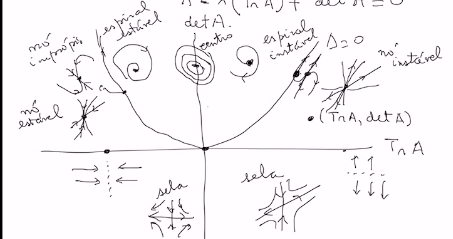
\includegraphics{edo1.png}
    \caption{edo1}
    \label{fig:my_label}
\end{figure}


\section{Sistemas Lineares não homogêneos (26/05)}
\begin{theorem}
    Dado o sistema não homogêneo $X' = AX + B(t)$, a solução do sistema é $X(t) = X_h(t) + X_p(t)$ onde $X_h(t)$ é solução da equação homogênea ($X' = A X$) e $X_p(t)$ é uma solução particular do sistema.
    
    Onde, a solução particular é tal que
    
    $$X_p(t) = e^{t A} \left [ \int_0^t e^{- A s} B(s) d s + K \right ], \ K \in \mathbb{R}^n$$
\end{theorem}

\section{Sistema não linear (31/05)}
\begin{lemma}
    Os pontos de equilíbrio do sistema não linear
    
    $$ \left \{
    \begin{array}{ll}
        x' = F(x, y) \\
        y' = G(x, y)
    \end{array} \right .
    $$
    
    É dado por $(x_0, y_0)$ tal que $F(x_0, y_0) = G(x_0, y_0) = 0$ 
\end{lemma}

\begin{theorem}
    Sejam $F(x, y)$ e $G(x, y)$ funções cujas derivadas parciais de segunda ordem são continuas. Então o sistema
    
    $$ \left \{
    \begin{array}{ll}
        x' = F(x, y) \\
        y' = G(x, y)
    \end{array} \right .
    $$
    
    É bem aproximado na vizinhança do ponto crítico $x_0, y_0)$ pelo sistema linear
    
    $$ \left \{
    \begin{array}{ll}
        x' = a x + b y \\
        y' = c x + d y
    \end{array} \right .
    $$
    
    onde $\left [ \begin{array}{cc}
        a & b \\
        c & d
    \end{array} \right ]$ é Jacobiano de $F(x, y)$ e $G(x, y)$ no ponto $(x_0, y_0)$
\end{theorem}

\section{Pendulo e Predador x Presa (02/06)}
Aula de aplicações.

\end{document}
